\vspace{-1em}
\begin{figure}[H]
    \centering
    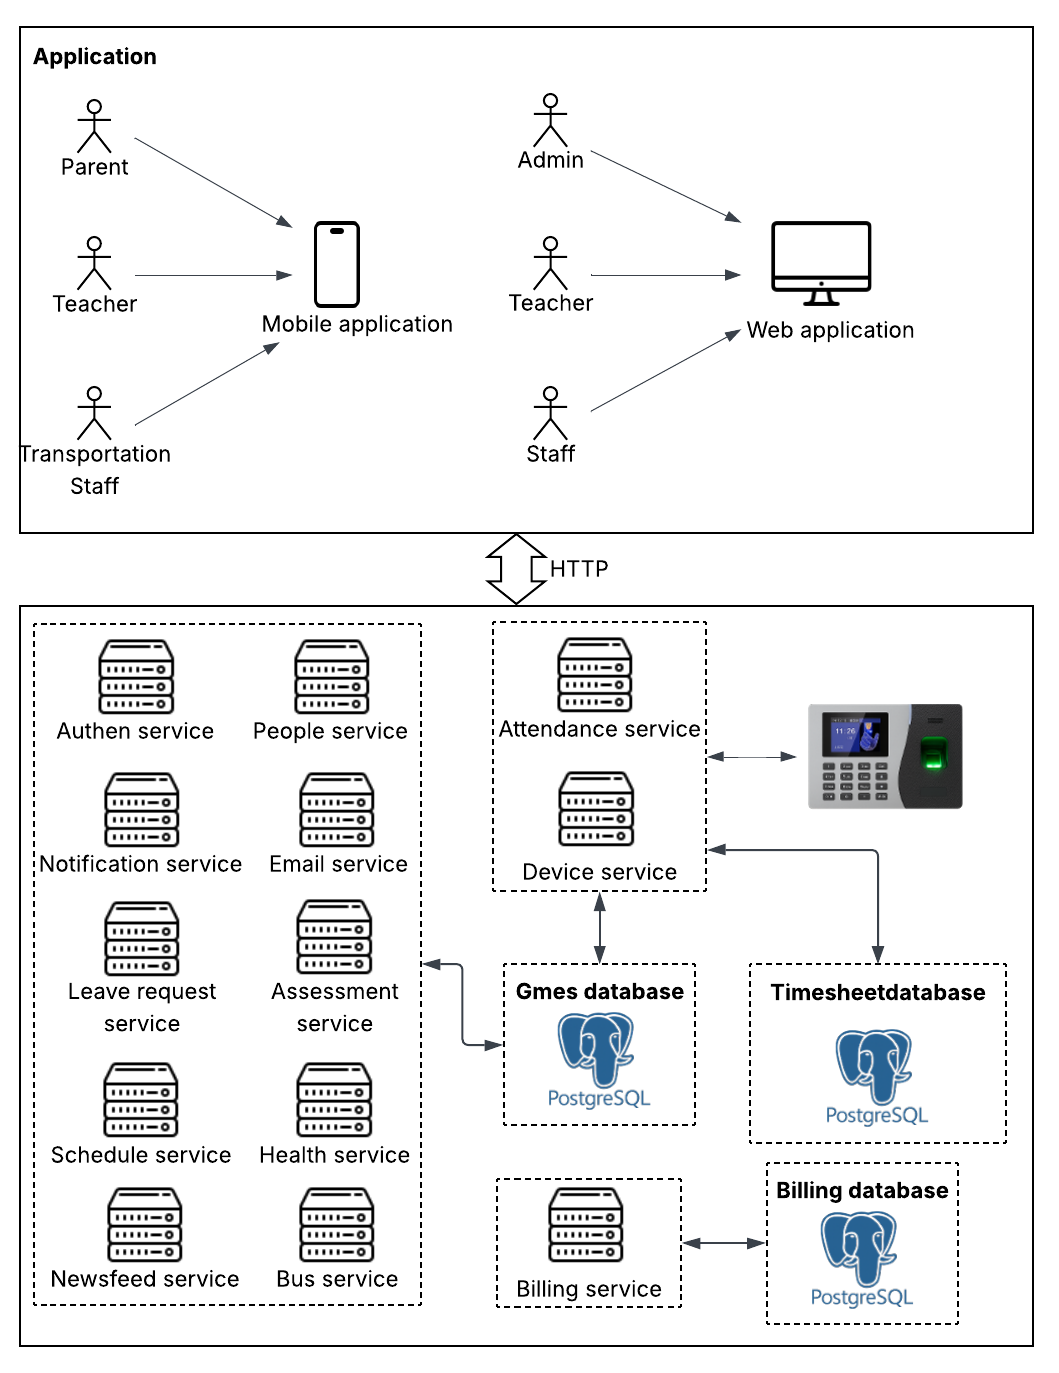
\includegraphics[width=0.9\textwidth]{images/sad_overview.png}
    \vspace{-1em}
    \caption{System architecture overview.}
    \label{fig:system_architecture_diagram_overview}
\end{figure}
\begin{minipage}{\textwidth}
    \setlength{\parindent}{2em}
   As shown in \textbf{\autoref{fig:system_architecture_diagram_overview}} the comprehensive overview of system architecture, the system provides both web and mobile application for differences user roles. These apps communicate with the server using the HTTP protocol, ensuring secure and reliable data exchange.

   Since GMES School is a comprehensive system handling multiple complex operations, it is designed using a microservices architecture. This approach allows each service to be developed, deployed, and scaled independently.
   
   Furthermore, to mange and stored data for these services, three separate PostgreSQL relational databases is designed:
\end{minipage}\\
\vspace{-0.8em}
\begin{itemize}
\setlength{\itemsep}{-0.1cm}
    \item A \textbf{GMES database} for core school data
    \item A \textbf{Timesheet database} for attendance data
    \item A \textbf{Billing database} for financial operations
\end{itemize}

\vspace{-0.5em}
\indent Futhermore, the system also integrates with physical attendance machines to accurately record  employee check-ins and check-outs time.
